\chapter{סוכנים אוטונומיים -- מ-\en{Chatbot} לעובד דיגיטלי}
\label{ch:autonomous-agents}

\begin{center}
\large\textbf{מטרות למידה}
\end{center}

\begin{itemize}
    \item \he{הבנת ההבדל בין צ'אטבוט פשוט לסוכן אוטונומי}
    \item \he{היכרות עם כלי Agentic Automation}
    \item \he{יכולת לתכנן ולנהל צוותים של סוכנים}
\end{itemize}

\section{הקדמה: מהפכת הסוכנים האוטונומיים}

\he{בשנת 2022, כאשר ChatGPT פרץ לתודעה הציבורית, רבים חשבו שהגענו לשיא היכולות של בינה מלאכותית שיחתית. אך כפי שקורה לעתים קרובות בהיסטוריה האנושית, מה שנראה כנקודת סיום התברר כנקודת פתיחה. הצ'אטבוטים, ככל שהיו מתוחכמים, היו מוגבלים למתן תשובות ישירות לשאלות ישירות. הם דמו למומחה נאמן שיושב מולנו ומחכה לשאלה הבאה - אך הוא אינו יוזם, אינו מתכנן, ואינו פועל באופן עצמאי.}

\he{ואז החלה התפתחות מרתקת: הופעת הסוכנים האוטונומיים~\cite{wang2023survey,xi2023rise}. בניגוד לצ'אטבוט מסורתי, סוכן אוטונומי הוא ישות דיגיטלית המסוגלת לקבל משימה כללית, לפרק אותה למשימות משנה, לתכנן דרך פעולה, לבצע את הפעולות הללו בסביבה אמיתית, וללמוד מהתוצאות. זוהי למעשה הקפיצה מעוזר וירטואלי לעובד דיגיטלי.}

\he{פרק זה יוביל אתכם במסע מהמהפכה הזאת - מהבנת ההבדלים הבסיסיים בין צ'אטבוט לסוכן, דרך היכרות עם הכלים והטכנולוגיות המובילות, ועד לתכנון ויישום של סוכנים אוטונומיים בארגון שלכם. נבחן כיצד לבנות צוותי סוכנים, כיצד למדוד את ערכם העסקי, וכיצד לפקח עליהם באופן שמבטיח ערך מקסימלי ומזעור סיכונים.}

\section{מצ'אטבוט לסוכן: מה השתנה?}

\subsection{הצ'אטבוט המסורתי: מגבלות וחוזקות}

\he{כדי להבין את המהפכה, עלינו תחילה להבין את המוצא. צ'אטבוט מסורתי - גם כזה שמבוסס על מודלי שפה מתקדמים - פועל במודל פשוט יחסית:}

\begin{enumerate}
    \item \he{המשתמש מכניס שאלה או בקשה}
    \item \he{המודל מעבד את הקלט}
    \item \he{המודל מייצר תשובה}
    \item \he{התשובה מוצגת למשתמש}
    \item \he{האינטראקציה מסתיימת}
\end{enumerate}

\he{מודל זה מצוין לתרחישים רבים: מענה על שאלות, סיכום טקסטים, ייעוץ מקצועי בסיסי. אך הוא סובל ממגבלות מהותיות:}

\begin{itemize}
    \item \textbf{\he{חוסר יוזמה}}: \he{הצ'אטבוט לא יכול להתחיל משימה בעצמו או להציע פעולה מבלי שנשאל}
    \item \textbf{\he{העדר זיכרון פעיל}}: \he{כל שיחה נפרדת; אין למידה או השבחה לאורך זמן}
    \item \textbf{\he{ללא יכולת ביצוע}}: \he{הצ'אטבוט יכול להמליץ לשלוח אימייל, אך לא לשלוח אותו בפועל}
    \item \textbf{\he{חוסר הקשר רחב}}: \he{האינטראקציה מבודדת, ללא קשר למערכות או תהליכים ארגוניים}
\end{itemize}

\subsection{הסוכן האוטונומי: פריצת דרך קונספטואלית}

\he{סוכן אוטונומי מייצג שינוי פרדיגמה. במקום מודל תגובתי, אנו מקבלים מודל יזום. במקום כלי עזר, אנו מקבלים שותף עבודה דיגיטלי. ההבדלים המרכזיים:}

\begin{itemize}
    \item \textbf{\he{תכנון אוטונומי}}: \he{הסוכן מקבל יעד כללי ומתכנן בעצמו את שלבי הפעולה}
    \item \textbf{\he{ביצוע בסביבה אמיתית}}: \he{הסוכן מתממשק עם \en{API}, מערכות ארגוניות, בסיסי נתונים}
    \item \textbf{\he{לולאת משוב}}: \he{הסוכן בודק את תוצאות פעולותיו ומתאים את התכנית בהתאם}
    \item \textbf{\he{למידה והשבחה}}: \he{ביצועי הסוכן משתפרים עם הזמן והניסיון}
    \item \textbf{\he{רב-שלביות}}: \he{הסוכן יכול לבצע סדרת פעולות מורכבת לאורך זמן}
\end{itemize}

\subsection{דיאגרמת השוואה: \en{Chatbot} לעומת \en{Agent} לעומת \en{Autonomous Agent}}

\he{איור~\ref{fig:chatbot-vs-agent} ממחיש את ההבדלים המהותיים בין שלוש רמות האוטומציה השיחתית. שימו לב לעלייה המשמעותית במורכבות ובאוטונומיה ככל שמתקדמים מצ'אטבוט פשוט לסוכן אוטונומי מלא.}

\begin{english}
\begin{figure}[h]
\centering
\begin{tikzpicture}[
    node distance=2cm,
    every node/.style={font=\footnotesize},
    box/.style={rectangle, draw, minimum width=3.5cm, minimum height=1.2cm, align=center, font=\small},
    arrow/.style={->, >=stealth, thick}
]

% Chatbot column
\node[box, fill=blue!10] (cb-input) at (0,0) {User Input};
\node[box, fill=blue!20] (cb-process) at (0,-2) {Processing};
\node[box, fill=blue!30] (cb-output) at (0,-4) {Output to User};
\node[above=0.3cm of cb-input, font=\bfseries] {Chatbot};

\draw[arrow] (cb-input) -- (cb-process);
\draw[arrow] (cb-process) -- (cb-output);

% Agent column
\node[box, fill=green!10] (ag-goal) at (5,0) {Goal};
\node[box, fill=green!20] (ag-plan) at (5,-1.2) {Planning};
\node[box, fill=green!25] (ag-exec) at (5,-2.4) {Execute Action};
\node[box, fill=green!30] (ag-check) at (5,-3.6) {Check Result};
\node[box, fill=green!35] (ag-decide) at (5,-4.8) {Decision};
\node[above=0.3cm of ag-goal, font=\bfseries] {Agent};

\draw[arrow] (ag-goal) -- (ag-plan);
\draw[arrow] (ag-plan) -- (ag-exec);
\draw[arrow] (ag-exec) -- (ag-check);
\draw[arrow] (ag-check) -- (ag-decide);
\draw[arrow] (ag-decide.east) -- ++(1,0) |- (ag-plan.east) node[midway, right, font=\tiny] {Not done};
\draw[arrow] (ag-decide) -- ++(0,-0.8) node[below, font=\small] {Done};

% Autonomous Agent column
\node[box, fill=orange!10] (aa-mission) at (10.5,0) {General Mission};
\node[box, fill=orange!15] (aa-decompose) at (10.5,-1.2) {Decompose to Subtasks};
\node[box, fill=orange!20] (aa-multiagent) at (10.5,-2.4) {Activate Other Agents};
\node[box, fill=orange!25] (aa-monitor) at (10.5,-3.6) {Monitor \& Control};
\node[box, fill=orange!30] (aa-learn) at (10.5,-4.8) {Learn \& Improve};
\node[above=0.3cm of aa-mission, font=\bfseries] {Autonomous Agent};

\draw[arrow] (aa-mission) -- (aa-decompose);
\draw[arrow] (aa-decompose) -- (aa-multiagent);
\draw[arrow] (aa-multiagent) -- (aa-monitor);
\draw[arrow] (aa-monitor) -- (aa-learn);
\draw[arrow] (aa-learn.east) -- ++(0.8,0) |- (aa-decompose.east) node[midway, right, font=\tiny] {Improve};

\end{tikzpicture}
\end{english}
\caption{השוואה בין שלושת רמות האוטומציה השיחתית}
\label{fig:chatbot-vs-agent}
\end{figure}

\subsection{מקרה בוחן: מתזמון פגישה ידני לאוטונומי מלא}

\he{כדי להמחיש את ההבדל, נבחן תרחיש עסקי פשוט: תזמון פגישה עם לקוח פוטנציאלי.}

\textbf{\he{תרחיש צ'אטבוט:}}
\begin{quote}
\he{מנהל מכירות: "אני צריך לתזמן פגישה עם ליאור כהן מחברת \en{XYZ}"}\\
\he{צ'אטבוט: "אני ממליץ לשלוח אימייל ולהציע \en{3} מועדים אפשריים. האם תרצה שאנסח עבורך את האימייל?"}\\
\he{מנהל מכירות: "כן"}\\
\he{צ'אטבוט: [מציג טיוטת אימייל]}\\
\he{מנהל מכירות: [צריך להעתיק, להדביק, לשלוח ידנית]}
\end{quote}

\textbf{\he{תרחיש סוכן אוטונומי:}}
\begin{quote}
\he{מנהל מכירות: "תזמן לי פגישה עם ליאור כהן מחברת \en{XYZ} השבוע הבא"}\\
\he{הסוכן האוטונומי:}
\begin{enumerate}
    \item \he{בודק ביומן של המנהל מתי יש זמינות}
    \item \he{מחפש ב-\en{CRM} את פרטי הקשר של ליאור כהן}
    \item \he{שולח אימייל עם \en{3} הצעות זמן}
    \item \he{ממתין לתשובה}
    \item \he{מזמין את הפגישה ביומן של שני הצדדים}
    \item \he{שולח אישור ומצרף חומרי רקע}
    \item \he{יומיים לפני הפגישה - שולח תזכורת}
\end{enumerate}
\he{מנהל מכירות: [לא צריך לעשות דבר]}
\end{quote}

\he{ההבדל הוא דרמטי. הצ'אטבוט חוסך זמן בניסוח, הסוכן האוטונומי חוסך את כל התהליך.}

\section{\en{Agentic AI}: הגדרה ועקרונות}

\subsection{הגדרה פורמלית}

\he{Agentic AI מתייחס למערכות בינה מלאכותית המציגות אוטונומיה, היכולת להגדיר יעדים, לתכנן פעולות, לבצע אותן בסביבה, וללמוד מהתוצאות~\cite{mialon2023augmented}. בניגוד למודלים סטטיים, מערכות Agentic מתאפיינות ביכולת לפעול לאורך זמן, להשתמש בכלים חיצוניים, ולהתאים את התנהגותן בהתאם למשוב מהסביבה~\cite{yao2022react}.}

\subsection{העקרונות המרכזיים של \en{Agentic AI}}

\subsubsection{תכנון (\en{Planning})}

\he{הסוכן האוטונומי אינו פועל באופן אימפולסיבי. הוא מקבל יעד ומפרק אותו לרצף של צעדים הגיוניים. תהליך התכנון כולל:}

\begin{itemize}
    \item \textbf{\he{פירוק משימה}}: \he{המרת יעד כללי למשימות קונקרטיות}
    \item \textbf{\he{סדר ביצוע}}: \he{קביעת סדר לוגי של פעולות}
    \item \textbf{\he{תלויות}}: \he{זיהוי איזה צעד תלוי בהשלמת צעד אחר}
    \item \textbf{\he{הקצאת משאבים}}: \he{קביעה אילו כלים או מערכות נדרשים}
\end{itemize}

\he{דוגמה: סוכן שמקבל משימה "צור דוח מכירות חודשי" יתכנן:}
\begin{enumerate}
    \item \he{שליפת נתוני מכירות מבסיס הנתונים}
    \item \he{חישוב סטטיסטיקות מרכזיות}
    \item \he{יצירת ויזואליזציות}
    \item \he{כתיבת תובנות טקסטואליות}
    \item \he{עיצוב מסמך \en{PDF}}
    \item \he{שליחת הדוח למנהלים הרלוונטיים}
\end{enumerate}

\subsubsection{ביצוע (\en{Execution})}

\he{לאחר התכנון, הסוכן מבצע את הפעולות בפועל. כאן טמון ההבדל המהותי מצ'אטבוט - הסוכן לא רק מציע מה לעשות, אלא עושה. ביצוע כולל:}

\begin{itemize}
    \item \textbf{\he{קריאות \en{API}}}: \he{התממשקות עם מערכות חיצוניות}
    \item \textbf{\he{מניפולציה של נתונים}}: \he{עריכה, עיבוד, המרה}
    \item \textbf{\he{יצירת תוצרים}}: \he{קבצים, הודעות, עדכונים במערכות}
    \item \textbf{\he{תקשורת}}: \he{שליחת אימיילים, הודעות, עדכונים}
\end{itemize}

\he{חשוב להבין: הסוכן פועל בסביבה אמיתית, לא סימולטיבית. כאשר הוא שולח אימייל - האימייל באמת נשלח. כאשר הוא מעדכן \en{CRM} - הרשומה באמת מתעדכנת. זו גם ההזדמנות וגם הסיכון.}

\subsubsection{למידה (\en{Learning})}

\he{הסוכן המתקדם לא רק מבצע משימות - הוא משתפר. למידה יכולה להתבצע במספר דרכים:}

\begin{itemize}
    \item \textbf{\he{למידה מהצלחות וכשלונות}}: \he{ניתוח מה עבד ומה לא}
    \item \textbf{\he{אופטימיזציה של תכנון}}: \he{מציאת דרכים יעילות יותר}
    \item \textbf{\he{התאמה אישית}}: \he{למידת העדפות של משתמשים ספציפיים}
    \item \textbf{\he{עדכון מודלים}}: \he{\en{Fine-tuning} של המודל הבסיסי}
\end{itemize}

\he{לדוגמה, סוכן שמזמן פגישות ילמד שמנהל מסוים מעדיף פגישות בשעות הבוקר, או שלקוחות מתעשייה מסוימת מעדיפים תקשורת פורמלית יותר.}

\subsubsection{משוב ובקרה (\en{Feedback \& Control})}

\he{אולי העיקרון החשוב ביותר - הסוכן לא פועל בלופ סגור. הוא כולל מנגנוני בקרה ומשוב:}

\begin{itemize}
    \item \textbf{\he{אימות תוצאות}}: \he{בדיקה שכל צעד הושלם בהצלחה}
    \item \textbf{\he{טיפול בשגיאות}}: \he{זיהוי כשלים ופעולות חלופיות}
    \item \textbf{\he{הסלמה לבני אדם}}: \he{ידיעה מתי להעביר שליטה לאדם}
    \item \textbf{\he{דיווח והתראות}}: \he{עדכון בזמן אמת על סטטוס}
\end{itemize}

\subsection{ארכיטקטורת הסוכן: מבט פנימה}

\he{כדי להבין כיצד סוכן אוטונומי עובד, נבחן את הארכיטקטורה הבסיסית. איור~\ref{fig:agent-architecture} מציג את הרכיבים המרכזיים ואת הקשרים ביניהם~\cite{sumers2024cognitive,xi2023rise}:}

\begin{english}
\begin{figure}[h]
\centering
\begin{tikzpicture}[
    node distance=1.5cm,
    box/.style={rectangle, draw, rounded corners, minimum width=3cm, minimum height=1cm, align=center, font=\small},
    arrow/.style={->, >=stealth, thick}
]

% Core LLM
\node[box, fill=purple!20] (llm) {Language Model\\(LLM Core)};

% Surrounding components
\node[box, fill=blue!20, above=of llm] (planning) {Planning Engine};
\node[box, fill=green!20, right=of llm] (memory) {Memory};
\node[box, fill=orange!20, below=of llm] (tools) {Tools\\(APIs, Tools)};
\node[box, fill=red!20, left=of llm] (monitor) {Monitor \& Control};

% External
\node[box, fill=gray!10, below=of tools] (external) {External Environment\\(CRM, Email, DB)};

% Arrows
\draw[arrow, <->] (llm) -- (planning);
\draw[arrow, <->] (llm) -- (memory);
\draw[arrow, <->] (llm) -- (tools);
\draw[arrow, <->] (llm) -- (monitor);
\draw[arrow, <->] (tools) -- (external);

\end{tikzpicture}
\end{english}
\caption{ארכיטקטורת סוכן אוטונומי}
\label{fig:agent-architecture}
\end{figure}

\he{כל רכיב ממלא תפקיד חיוני:}

\begin{itemize}
    \item \textbf{\he{מודל השפה (\en{LLM Core})}}: \he{המוח - מבין הנחיות, מקבל החלטות, מייצר תוכן}
    \item \textbf{\he{מנוע תכנון}}: \he{פורק משימות ומתווה דרכי פעולה}
    \item \textbf{\he{זיכרון}}: \he{שומר הקשר, היסטוריה, למידה}
    \item \textbf{\he{כלים}}: \he{מאפשרים ביצוע פעולות בעולם האמיתי}
    \item \textbf{\he{ניטור ובקרה}}: \he{מבטיח פעולה בטוחה ומדווחת}
\end{itemize}

\section{כלי \en{Agentic Automation}: מפת הטכנולוגיות}

\he{עולם ה-Agentic Automation מתפתח במהירות מסחררת. בשנים האחרונות צצו עשרות כלים, פלטפורמות ופריימוורקים שמאפשרים בניה של סוכנים אוטונומיים. נחלק אותם לשלוש קטגוריות עיקריות:}

\subsection{פריימוורקים מבוססי קוד: \en{LangGraph} ו-\en{AutoGen}}

\subsubsection{\en{LangGraph}: תזמור סוכנים מורכבים}

\he{LangGraph~\cite{langgraph2024}, חלק ממשפחת LangChain~\cite{langchain2023}, הוא פריימוורק המאפשר לבנות workflows מורכבים של סוכנים. הרעיון המרכזי: ייצוג התהליך כגרף, כאשר כל צומת היא פעולה או החלטה.}

\textbf{\he{מתי להשתמש ב-LangGraph:}}
\begin{itemize}
    \item \he{תהליכים מורכבים עם נתיבים מרובים}
    \item \he{צורך בשליטה מלאה על ה-workflow}
    \item \he{אינטגרציה עמוקה עם Python ecosystem}
    \item \he{בניית סוכנים מתקדמים עם state management}
\end{itemize}

\textbf{\he{יתרונות:}}
\begin{itemize}
    \item \he{גמישות מקסימלית}
    \item \he{תמיכה ב-streaming ו-async}
    \item \he{דיבוגינג וויזואליזציה של הגרף}
    \item \he{קהילה גדולה ותיעוד מצוין}
\end{itemize}

\textbf{\he{חסרונות:}}
\begin{itemize}
    \item \he{עקומת למידה תלולה}
    \item \he{דורש ידע בתכנות}
    \item \he{זמן פיתוח ארוך יותר}
\end{itemize}

\subsubsection{\en{AutoGen}: צוותי סוכנים בשיחה}

\he{AutoGen~\cite{wu2023autogen,autogen2023}, פיתוח של Microsoft Research, לוקח גישה שונה: הוא מדמה שיחות בין סוכנים שונים, כאשר כל סוכן מייצג תפקיד או מומחיות. הרעיון: פתרון בעיות מורכבות דרך דיאלוג בין סוכנים.}

\textbf{\he{מתי להשתמש ב-AutoGen:}}
\begin{itemize}
    \item \he{משימות שדורשות מומחיות מרובה}
    \item \he{תהליכי בדיקה ואימות}
    \item \he{כתיבת קוד עם code review אוטומטי}
    \item \he{סימולציה של דיונים וקבלת החלטות}
\end{itemize}

\textbf{\he{יתרונות:}}
\begin{itemize}
    \item \he{מודל אינטואיטיבי של שיחה}
    \item \he{מובנה למשימות תכנות}
    \item \he{קל יחסית ליישום}
    \item \he{תוצאות מרשימות במשימות מורכבות}
\end{itemize}

\textbf{\he{חסרונות:}}
\begin{itemize}
    \item \he{צריכה גבוהה של tokens}
    \item \he{קשה לחזות את משך הריצה}
    \item \he{פחות שליטה על התהליך המדויק}
\end{itemize}

\subsection{פלטפורמות \en{Low-Code}: \en{n8n} ו-\en{Zapier}}

\subsubsection{n8n: אוטומציה עם גמישות}

\he{n8n~\cite{n8n2024workflow} הוא כלי workflow automation בעל קוד פתוח, עם ממשק ויזואלי לבניית אוטומציות. הוא מצטיין באינטגרציות רבות ויכולות מתקדמות.}

\textbf{\he{מתי להשתמש ב-\en{n8n}:}}
\begin{itemize}
    \item \he{אוטומציה של תהליכים עסקיים רגילים}
    \item \he{צורך באינטגרציות עם מערכות רבות}
    \item \he{רצון לשלוט על הדאטה (\en{self-hosted})}
    \item \he{צוות ללא רקע תכנותי מעמיק}
\end{itemize}

\textbf{\he{יתרונות:}}
\begin{itemize}
    \item \he{ממשק ויזואלי אינטואיטיבי}
    \item \he{למעלה מ-\en{300} אינטגרציות מובנות}
    \item \he{קוד פתוח - ניתן ל-\en{self-host}}
    \item \he{תמיכה ב-\en{custom code} (\en{JavaScript/Python})}
    \item \he{מחיר תחרותי}
\end{itemize}

\textbf{\he{חסרונות:}}
\begin{itemize}
    \item \he{ממשק משתמש פחות מלוטש מהמתחרים}
    \item \he{תיעוד לא תמיד מקיף}
    \item \he{ביצועים יכולים להיות איטיים ב-\en{workflows} מורכבים}
\end{itemize}

\subsubsection{\en{Zapier}: פשטות ומהירות}

\he{\en{Zapier}~\cite{zapier2024} הוא הוותיק בתחום - פלטפורמת אוטומציה המחברת בין אפליקציות שונות בקלות. הפילוסופיה: אוטומציה צריכה להיות פשוטה כמו בניית \en{LEGO}.}

\textbf{\he{מתי להשתמש ב-Zapier:}}
\begin{itemize}
    \item \he{אוטומציות פשוטות עד בינוניות}
    \item \he{צורך בהקמה מהירה}
    \item \he{שימוש באפליקציות \en{SaaS} פופולריות}
    \item \he{צוות לא טכני}
\end{itemize}

\textbf{\he{יתרונות:}}
\begin{itemize}
    \item \he{קל ביותר לשימוש}
    \item \he{למעלה מ-\en{5,000} אינטגרציות}
    \item \he{אמינות ויציבות גבוהות}
    \item \he{תמיכת לקוחות מצוינת}
    \item \he{\en{Templates} מוכנים לשימוש}
\end{itemize}

\textbf{\he{חסרונות:}}
\begin{itemize}
    \item \he{יקר ב-\en{scale}}
    \item \he{מוגבל ב-\en{workflows} מורכבים}
    \item \he{פחות גמישות}
    \item \he{לא ניתן ל-\en{self-host}}
\end{itemize}

\subsection{פלטפורמות \en{Zero-Code}: \en{Make}, \en{RelevanceAI}, \en{Google AI Studio}}

\subsubsection{Make (Integromat לשעבר): אוטומציה ויזואלית}

\he{Make~\cite{make2024} מציע ממשק ויזואלי מתקדם במיוחד, המאפשר בניית אוטומציות מורכבות ללא כתיבת קוד. הוא מצטיין בטיפול בנתונים ובנתיבים מסועפים.}

\textbf{\he{מתי להשתמש ב-Make:}}
\begin{itemize}
    \item \he{workflows מורכבים עם לוגיקה מסועפת}
    \item \he{טיפול בנפחי דאטה גבוהים}
    \item \he{צורך בויזואליזציה ברורה של התהליך}
    \item \he{צוות שמעריך עיצוב ו-\en{UX}}
\end{itemize}

\textbf{\he{יתרונות:}}
\begin{itemize}
    \item \he{ממשק ויזואלי מצוין}
    \item \he{טיפול מתקדם בדאטה (\en{arrays, JSON, transformations})}
    \item \he{מודל תמחור צודק יותר (לפי operations)}
    \item \he{יכולות debugging טובות}
\end{itemize}

\textbf{\he{חסרונות:}}
\begin{itemize}
    \item \he{עקומת למידה בינונית}
    \item \he{פחות אינטגרציות מ-Zapier}
    \item \he{תיעוד לא תמיד מספיק}
\end{itemize}

\subsubsection{\en{RelevanceAI}: סוכני \en{AI} מותאמים אישית}

\he{RelevanceAI~\cite{relevanceai2024} מתמקד ספציפית בבניית סוכני AI - ממשק שמאפשר ליצור סוכנים מותאמים לתהליכים עסקיים ספציפיים, עם אינטגרציות לכלי עבודה נפוצים.}

\textbf{\he{מתי להשתמש ב-\en{RelevanceAI}:}}
\begin{itemize}
    \item \he{בניית סוכנים ממוקדי \en{AI}}
    \item \he{תהליכים שדורשים הבנת שפה טבעית}
    \item \he{אוטומציות של מחקר ואיסוף מידע}
    \item \he{צוות שרוצה להתמקד בלוגיקה עסקית, לא בטכנולוגיה}
\end{itemize}

\textbf{\he{יתרונות:}}
\begin{itemize}
    \item \he{ממוקד לסוכני \en{AI}}
    \item \he{קל ליצור סוכנים מתקדמים}
    \item \he{תבניות מוכנות לתהליכים נפוצים}
    \item \he{אינטגרציה טובה עם \en{LLMs}}
\end{itemize}

\textbf{\he{חסרונות:}}
\begin{itemize}
    \item \he{פלטפורמה חדשה יחסית}
    \item \he{קהילה קטנה}
    \item \he{פחות אינטגרציות ממתחרים גדולים}
\end{itemize}

\subsubsection{\en{Google AI Studio}: יצירה מהירה של אפליקציות \en{AI}}

\he{\en{Google AI Studio} הוא סביבת פיתוח מהירה לבניית אפליקציות המשתמשות במודלי \en{Gemini} של \en{Google}. הוא מציע ממשק פשוט ליצירת \en{prompts}, פונקציות וסוכנים בסיסיים.}

\textbf{\he{מתי להשתמש ב-\en{Google AI Studio}:}}
\begin{itemize}
    \item \he{פרוטוטייפינג מהיר}
    \item \he{שימוש במודלי \en{Gemini}}
    \item \he{אפליקציות פשוטות יחסית}
    \item \he{אקוסיסטם \en{Google} (\en{Workspace, Cloud})}
\end{itemize}

\textbf{\he{יתרונות:}}
\begin{itemize}
    \item \he{חינמי לשימוש בסיסי}
    \item \he{קל מאוד להתחיל}
    \item \he{אינטגרציה חלקה עם \en{Google Cloud}}
    \item \he{גישה למודלי \en{Gemini} המתקדמים}
\end{itemize}

\textbf{\he{חסרונות:}}
\begin{itemize}
    \item \he{מוגבל למודלי Google בלבד}
    \item \he{אינטגרציות מוגבלות}
    \item \he{פחות מתאים לאוטומציות מורכבות}
\end{itemize}

\subsection{טבלת השוואה: מציאת הכלי המתאים}

\he{טבלה~\ref{tab:tools-comparison} מסכמת את ההשוואה בין הכלים המובילים לפי קריטריונים מרכזיים, ומאפשרת לבחור את הכלי המתאים לצרכים הספציפיים של הארגון.}

\begin{table}[h]
\centering
\small
\begin{rtltabular}{|p{2.5cm}|c|c|c|c|c|}
\hline
\hebheader{קריטריון} & \textbf{\textenglish{LangGraph}} & \textbf{\textenglish{n8n}} & \textbf{\textenglish{Zapier}} & \textbf{\textenglish{Make}} & \textbf{\textenglish{RelevanceAI}} \\
\hline
\hebcell{דרישת תכנות} & \hebcell{גבוהה} & \hebcell{נמוכה} & \hebcell{אפס} & \hebcell{אפס} & \hebcell{אפס} \\
\hline
\hebcell{גמישות} & \textenglish{5/5} & \textenglish{4/5} & \textenglish{2/5} & \textenglish{3/5} & \textenglish{3/5} \\
\hline
\hebcell{קלות שימוש} & \textenglish{2/5} & \textenglish{3/5} & \textenglish{5/5} & \textenglish{4/5} & \textenglish{4/5} \\
\hline
\hebcell{אינטגרציות} & \hebcell{בעצמך} & \textenglish{300+} & \textenglish{5000+} & \textenglish{1500+} & \textenglish{100+} \\
\hline
\hebcell{מחיר יחסי} & \hebcell{נמוך} & \hebcell{בינוני} & \hebcell{גבוה} & \hebcell{בינוני} & \hebcell{גבוה} \\
\hline
\hebcell{מורכבות מקס׳} & \hebcell{אין גבול} & \hebcell{גבוהה} & \hebcell{בינונית} & \hebcell{גבוהה} & \hebcell{בינונית} \\
\hline
\hebcell{זמן ל-\textenglish{POC}} & \hebcell{שבועות} & \hebcell{ימים} & \hebcell{שעות} & \hebcell{ימים} & \hebcell{ימים} \\
\hline
\end{rtltabular}
\caption{השוואת כלי \textenglish{Agentic Automation} מובילים}
\label{tab:tools-comparison}
\end{table}

\section{תכנון \en{Workflow} לסוכנים}

\he{בניית סוכן אוטונומי אפקטיבי אינה עניין טכני בלבד - היא דורשת תכנון מתודי של ה-workflow. תכנון גרוע יביא לסוכן שלא עובד, בזבז משאבים, או גרוע מכך - גורם נזקים. תכנון טוב יוביל לסוכן שחוסך זמן, משפר תהליכים, ומספק ערך אמיתי.}

\subsection{שלבי תכנון \en{Workflow}}

\subsubsection{שלב 1: הגדרת המטרה והיקף}

\he{כל תכנון מתחיל בשאלה פשוטה אך מהותית: מה בדיוק הסוכן אמור להשיג? הגדרה מעורפלת תוביל לסוכן מעורפל.}

\textbf{\he{שאלות מנחות:}}
\begin{itemize}
    \item \he{מה הבעיה העסקית שהסוכן פותר?}
    \item \he{מהי ההגדרה של "הצלחה" עבור סוכן זה?}
    \item \he{מהן גבולות הסמכות של הסוכן? מה הוא יכול ומה הוא לא יכול לעשות?}
    \item \he{מתי הסוכן יועבר לבקרה אנושית?}
\end{itemize}

\textbf{\he{דוגמה - הגדרה גרועה:}}
\begin{quote}
\he{"סוכן שמטפל בלידים"}
\end{quote}

\textbf{\he{דוגמה - הגדרה טובה:}}
\begin{quote}
\he{"סוכן שמקבל ליד חדש מהאתר, מאמת שהוא איכותי (תקציב > \en{50K}, בתעשיות היעד), מעשיר אותו בנתונים מ-\en{LinkedIn} ו-\en{Clearbit}, מקצה אותו לאיש מכירות מתאים בהתאם לגיאוגרפיה ומומחיות, ושולח אימייל היכרות אישי. במקרה של ליד \en{VIP} (תקציב > \en{500K}) - מתריע למנהל מכירות בנוסף."}
\end{quote}

\subsubsection{שלב 2: מיפוי התהליך הנוכחי}

\he{לפני שבונים אוטומציה, יש להבין לעומק את התהליך הידני הקיים:}

\begin{enumerate}
    \item \he{מי מבצע את התהליך כיום?}
    \item \he{אילו שלבים הוא כולל?}
    \item \he{אילו מערכות מעורבות?}
    \item \he{אילו החלטות מתקבלות בדרך?}
    \item \he{מהם מקרי הקצה והחריגים?}
    \item \he{כמה זמן לוקח התהליך?}
    \item \he{מהם נקודות הכשל הנפוצות?}
\end{enumerate}

\he{כדאי לשבת עם מי שמבצע את התהליך היום ולמפות אותו צעד אחר צעד. תגלו לעתים קרובות שהתהליך מורכב יותר ממה שנראה מבחוץ.}

\subsubsection{שלב 3: פירוק למשימות ולצמתי החלטה}

\he{כעת יש לפרק את התהליך לרכיבים:}

\begin{itemize}
    \item \textbf{\he{פעולות}}: \he{צעדים קונקרטיים שהסוכן מבצע}
    \item \textbf{\he{צמתי החלטה}}: \he{נקודות שבהן הסוכן צריך לבחור בין מסלולים}
    \item \textbf{\he{אימותים}}: \he{בדיקות שהסוכן מבצע לפני המשך}
    \item \textbf{\he{טיפול בשגיאות}}: \he{מה קורה כאשר משהו משתבש}
\end{itemize}

\subsubsection{שלב 4: זיהוי תלויות ואילוצים}

\he{לא כל צעד יכול להתבצע בכל רגע:}

\begin{itemize}
    \item \he{אילו צעדים תלויים בהשלמת צעדים אחרים?}
    \item \he{האם יש אילוצי זמן? (למשל, לא לשלוח אימיילים בשבת)}
    \item \he{האם יש הגבלות על קצב ביצוע? (\en{rate limits} של \en{APIs})}
    \item \he{האם יש צורך באישורים חיצוניים?}
\end{itemize}

\subsubsection{שלב 5: תכנון טיפול בחריגים}

\he{הסוכן המעולה לא מוגדר רק על ידי מה שהוא עושה כאשר הכל עובד, אלא על ידי מה שהוא עושה כאשר דברים משתבשים:}

\begin{itemize}
    \item \he{מה קורה אם \en{API} לא עונה?}
    \item \he{מה קורה אם הנתונים שחזרו לא תקינים?}
    \item \he{מה קורה אם המשתמש נתן קלט לא תקין?}
    \item \he{כמה ניסיונות נעשה? מתי נכשל?}
    \item \he{מי צריך לקבל התראה במקרה של כשלון?}
\end{itemize}

\subsection{דיאגרמת \en{Workflow} מורכבת: ניהול לידים אוטומטי}

\he{איור~\ref{fig:lead-workflow} מציג דיאגרמת \en{workflow} מלאה לסוכן ניהול לידים, כולל צמתי החלטה, טיפול במקרים שונים, והמסלול המלא מליד חדש ועד עדכון \en{CRM}.}

\begin{english}
\begin{figure}[h]
\centering
\begin{tikzpicture}[
    node distance=1.3cm and 1.5cm,
    startstop/.style={rectangle, rounded corners, minimum width=2.5cm, minimum height=0.8cm, align=center, draw=black, fill=red!20, font=\tiny},
    process/.style={rectangle, minimum width=2.5cm, minimum height=0.8cm, align=center, draw=black, fill=blue!20, font=\tiny},
    decision/.style={diamond, minimum width=2cm, minimum height=1cm, align=center, draw=black, fill=green!20, font=\tiny, aspect=2},
    arrow/.style={thick,->,>=stealth}
]

% Start
\node[startstop] (start) {New Lead from Website};

% Process nodes
\node[process, below=of start] (extract) {Extract Basic Data};
\node[decision, below=of extract] (validate) {Valid?};
\node[process, right=of validate] (reject) {Send to Trash};
\node[process, below=of validate] (enrich) {Enrich from External APIs};
\node[decision, below=of enrich] (quality) {Quality?};
\node[process, below=of quality] (score) {Calculate Score};
\node[decision, below=of score] (vip) {VIP?};
\node[process, below left=of vip] (assign-vip) {Assign to Manager + Alert};
\node[process, below right=of vip] (assign-regular) {Assign to Regular Rep};
\node[process, below=1.5cm of vip] (email) {Send Opening Email};
\node[process, below=of email] (crm) {Update CRM};
\node[startstop, below=of crm] (end) {End};

% Arrows
\draw[arrow] (start) -- (extract);
\draw[arrow] (extract) -- (validate);
\draw[arrow] (validate) -- node[anchor=south, font=\tiny] {No} (reject);
\draw[arrow] (validate) -- node[anchor=east, font=\tiny] {Yes} (enrich);
\draw[arrow] (enrich) -- (quality);
\draw[arrow] (quality) -- node[anchor=south, font=\tiny] {No} ++(2,0) |- (reject);
\draw[arrow] (quality) -- node[anchor=east, font=\tiny] {Yes} (score);
\draw[arrow] (score) -- (vip);
\draw[arrow] (vip) -| node[near start, anchor=east, font=\tiny] {Yes} (assign-vip);
\draw[arrow] (vip) -| node[near start, anchor=west, font=\tiny] {No} (assign-regular);
\draw[arrow] (assign-vip) |- (email);
\draw[arrow] (assign-regular) |- (email);
\draw[arrow] (email) -- (crm);
\draw[arrow] (crm) -- (end);

\end{tikzpicture}
\end{english}
\caption{דיאגרמת \en{Workflow} לסוכן ניהול לידים אוטומטי}
\label{fig:lead-workflow}
\end{figure}

\subsection{עקרונות לתכנון \en{Workflow} אפקטיבי}

\subsubsection{עקרון המודולריות}

\he{בנו את ה-workflow בבלוקים עצמאיים שניתן לבדוק, לשנות ולעדכן בנפרד. אם חלק אחד משתבש, הוא לא יפיל את כל המערכת.}

\subsubsection{עקרון האידמפוטנטיות}

\he{וודאו שהפעלה חוזרת של אותה פעולה עם אותם נתונים לא תגרום לכפילויות או לבעיות. אם הסוכן נכשל באמצע ונצטרך להפעיל אותו שוב, הוא לא ישלח 5 אימיילים במקום 1.}

\subsubsection{עקרון הנראות (\en{Observability})}

\he{כל שלב צריך לרשום לוג ברור. בכל רגע צריך להיות אפשר לדעת:}
\begin{itemize}
    \item \he{איפה הסוכן נמצא בתהליך}
    \item \he{מה הוא עשה עד כה}
    \item \he{מה הולך לקרות הלאה}
\end{itemize}

\subsubsection{עקרון ה-\en{Fail Fast}}

\he{אם משהו לא יכול להצליח - תכשל מהר. אל תבזבז משאבים על המשך תהליך שכבר ידוע שייכשל.}

\subsubsection{עקרון ה-\en{Graceful Degradation}}

\he{אם חלק מהמערכת לא זמין - הסוכן ימשיך לתפקד ברמה מופחתת במקום להיכשל לגמרי. למשל, אם שירות העשרה נתונים לא עובד, הסוכן ימשיך עם הנתונים שיש לו.}

\section{ניטור ובקרה: פיקוח על סוכנים אוטונומיים}

\he{סוכן אוטונומי שפועל ללא פיקוח הוא מתכון לאסון. אך יותר מדי פיקוח מבטל את היתרונות של האוטומציה. המטרה: מציאת האיזון הנכון בין אוטונומיה לביקורת.}

\subsection{רמות הפיקוח}

\subsubsection{רמה 1: פיקוח מלא (\en{Human-in-the-Loop})}

\he{בכל צעד קריטי, הסוכן מבקש אישור אנושי לפני ביצוע.}

\textbf{\he{מתי להשתמש:}}
\begin{itemize}
    \item \he{שלבי פיתוח ראשוניים}
    \item \he{פעולות בעלות השלכות כלכליות משמעותיות}
    \item \he{תחומים רגולטוריים (בריאות, פיננסים)}
\end{itemize}

\textbf{\he{יתרונות:}} \he{בטיחות מקסימלית, למידה מהירה מהאדם}\\
\textbf{\he{חסרונות:}} \he{איטי, לא באמת אוטומטי}

\subsubsection{רמה 2: פיקוח סלקטיבי (\en{Human-on-the-Loop})}

\he{הסוכן פועל באופן אוטונומי, אך מעביר לאישור אנושי מקרים חריגים או בעלי סיכון גבוה.}

\textbf{\he{מתי להשתמש:}}
\begin{itemize}
    \item \he{סוכנים בשלבי בגרות בינוניים}
    \item \he{תהליכים שרוב המקרים שגרתיים אך יש חריגים}
    \item \he{איזון בין מהירות לבטיחות}
\end{itemize}

\textbf{\he{יתרונות:}} \he{איזון טוב, חיסכון זמן משמעותי}\\
\textbf{\he{חסרונות:}} \he{דורש הגדרה טובה של "חריג"}

\subsubsection{רמה 3: פיקוח בדיעבד (\en{Human-after-the-Loop})}

\he{הסוכן פועל באופן מלא אוטונומי, אך כל פעולה נרשמת ויכולה להיבדק בדיעבד.}

\textbf{\he{מתי להשתמש:}}
\begin{itemize}
    \item \he{סוכנים בוגרים ומוכחים}
    \item \he{פעולות בעלות סיכון נמוך}
    \item \he{נפחים גבוהים שלא מעשי לבדוק כל אחד}
\end{itemize}

\textbf{\he{יתרונות:}} \he{מהירות מקסימלית, חיסכון זמן אדיר}\\
\textbf{\he{חסרונות:}} \he{סיכון גבוה יותר, טעויות מתגלות רק בדיעבד}

\subsection{מטריקות ניטור חיוניות}

\he{כדי לפקח ביעילות על סוכנים, יש להגדיר מטריקות ברורות:}

\subsubsection{מטריקות ביצוע}

\begin{itemize}
    \item \textbf{\he{Success Rate}}: \he{אחוז המשימות שהסתיימו בהצלחה}
    \[
    \text{Success Rate} = \frac{\text{Successful Runs}}{\text{Total Runs}} \times 100
    \]

    \item \textbf{\he{Error Rate}}: \he{אחוז המשימות שנכשלו}
    \[
    \text{Error Rate} = \frac{\text{Errors}}{\text{Total Operations}} \times 100
    \]

    \item \textbf{\he{Average Execution Time}}: \he{זמן ביצוע ממוצע למשימה}

    \item \textbf{\he{Tasks per Hour/Day}}: \he{תפוקה}
\end{itemize}

\subsubsection{מטריקות עסקיות}

\begin{itemize}
    \item \textbf{\he{Time Saved}}: \he{שעות עבודה אנושיות שנחסכו}

    \item \textbf{\he{Cost per Operation}}: \he{עלות ממוצעת לפעולה}
    \[
    \text{Cost per Op} = \frac{\text{Total Cost (Dev + Run + Maintenance)}}{\text{Number of Operations}}
    \]

    \item \textbf{\he{\en{ROI}}}:
    \[
    \text{Automation ROI} = \frac{\text{Saved Human Hours} \times \text{Hourly Wage}}{\text{Dev Cost} + \text{Maintenance Cost}}
    \]

    \item \textbf{\he{\en{Quality Metrics}}}: \he{שיפור באיכות התוצרים (פחות שגיאות, זמן תגובה מהיר יותר)}
\end{itemize}

\subsubsection{מטריקות אמינות}

\begin{itemize}
    \item \textbf{\he{\en{Uptime}}}: \he{אחוז הזמן שהסוכן זמין ופועל}

    \item \textbf{\he{\en{Mean Time Between Failures (MTBF)}}}

    \item \textbf{\he{Mean Time to Recovery (MTTR)}}: \he{זמן ממוצע לתיקון כשלון}

    \item \textbf{\he{Retry Rate}}: \he{כמה פעולות דרשו ניסיון חוזר}
\end{itemize}

\subsection{כלים לניטור ולוגינג}

\subsubsection{לוגים מובנים}

\he{רוב פלטפורמות האוטומציה מספקות לוגים בסיסיים:}
\begin{itemize}
    \item \he{n8n: Execution logs עם סטטוס כל node}
    \item \he{Zapier: Task History עם פילטור ומיון}
    \item \he{Make: Execution history עם ויזואליזציה של הרצה}
\end{itemize}

\subsubsection{מערכות ניטור חיצוניות}

\he{לניטור מתקדם יותר, כדאי לשקול:}
\begin{itemize}
    \item \textbf{\en{Datadog / New Relic}}: \he{לניטור ביצועים ואלרטים}
    \item \textbf{\en{Sentry}}: \he{למעקב אחר שגיאות ו-\en{exceptions}}
    \item \textbf{\en{Grafana + Prometheus}}: \he{לויזואליזציה של מטריקות}
    \item \textbf{\en{ELK Stack (Elasticsearch, Logstash, Kibana)}}: \he{לניתוח לוגים מתקדם}
\end{itemize}

\subsection{אסטרטגיות התראה (\en{Alerting})}

\he{לא כדאי לקבל התראה על כל דבר - זה יוביל ל-\en{alert fatigue}. במקום זאת:}

\subsubsection{התראות קריטיות (\en{Critical Alerts})}

\he{שולחות מיד, 24/7:}
\begin{itemize}
    \item \he{הסוכן נפל לחלוטין ולא פועל}
    \item \he{שגיאה שגרמה לנזק כלכלי או תדמיתי}
    \item \he{פריצת אבטחה או גישה לא מורשית}
\end{itemize}

\subsubsection{התראות חשובות (\en{High Priority})}

\he{שולחות בשעות עבודה או בסיכום יומי:}
\begin{itemize}
    \item \he{אחוז שגיאות חצה סף מוגדר (למשל \en{5\%})}
    \item \he{זמן ביצוע עלה משמעותית}
    \item \he{מספר ניסיונות חוזרים גבוה מהרגיל}
\end{itemize}

\subsubsection{התראות מידע (\en{Info})}

\he{סיכום שבועי או חודשי:}
\begin{itemize}
    \item \he{סטטיסטיקות כלליות}
    \item \he{טרנדים לאורך זמן}
    \item \he{המלצות לשיפור}
\end{itemize}

\subsection{בקרת איכות ואימות}

\he{ניטור אינו רק בדיקה שהסוכן רץ - אלא גם שהוא עושה את הדבר הנכון:}

\subsubsection{\en{Spot Checks}}

\he{בדיקות מדגמיות קבועות:}
\begin{itemize}
    \item \he{כל שבוע - דגימה אקראית של 10-20 מקרים}
    \item \he{בדיקה ידנית: האם הפעולה שבוצעה הייתה נכונה?}
    \item \he{תיעוד ממצאים ותיקונים}
\end{itemize}

\subsubsection{\en{A/B Testing}}

\he{השוואה בין הסוכן לביצוע אנושי:}
\begin{itemize}
    \item \he{חלק מהמשימות מבוצעות על ידי הסוכן}
    \item \he{חלק על ידי בני אדם}
    \item \he{השוואת איכות, מהירות, עלות}
\end{itemize}

\subsubsection{\en{Regression Testing}}

\he{בכל עדכון של הסוכן:}
\begin{itemize}
    \item \he{הרצה על סט נתוני בדיקה קבוע}
    \item \he{וידוא שהשינויים לא פגעו ביכולות קיימות}
\end{itemize}

\section{דוגמאות מעשיות}

\subsection{דוגמה 1: סוכן לניהול לידים אוטומטי}

\subsubsection{רקע עסקי}

\he{חברת SaaS בגודל בינוני מקבלת כ-200 לידים חדשים בשבוע דרך האתר. התהליך הידני:}
\begin{enumerate}
    \item \he{צוות שיווק בודק את הלידים ידנית}
    \item \he{מעשיר נתונים מ-LinkedIn}
    \item \he{מדרג לפי התאמה}
    \item \he{מעביר למכירות}
    \item \he{נציג מכירות שולח אימייל פתיחה}
\end{enumerate}

\he{התהליך לוקח בממוצע 48 שעות ללילד, ודורש כ-15 שעות עבודה שבועיות.}

\subsubsection{הפתרון: סוכן אוטונומי}

\textbf{\he{טכנולוגיה:}} n8n + Airtable + Clearbit API + OpenAI API

\textbf{\he{תהליך:}}
\begin{enumerate}
    \item \textbf{\he{טריגר}}: \he{ליד חדש נכנס ל-\en{Airtable} (דרך \en{Webhook} מהאתר)}

    \item \textbf{\he{אימות בסיסי}}: \he{בדיקה שהשדות החובה מלאים (שם, אימייל, חברה)}

    \item \textbf{\he{העשרת נתונים}}:
    \begin{itemize}
        \item \he{\en{Clearbit Enrichment API} - גודל חברה, תעשייה, תקציב משוער}
        \item \he{\en{LinkedIn API} (דרך \en{PhantomBuster}) - תפקיד איש הקשר}
    \end{itemize}

    \item \textbf{\he{דירוג איכות}} (באמצעות \en{OpenAI}):
    \begin{itemize}
        \item \he{Prompt: "דרג ליד זה מ-1 עד 10 בהתאם לקריטריונים..."}
        \item \he{קריטריונים: גודל חברה, תעשייה, תפקיד, \en{budget signals}}
    \end{itemize}

    \item \textbf{\he{הקצאה לנציג}}:
    \begin{itemize}
        \item \he{אם ציון > \en{8}: הקצאה למנהל מכירות בכיר + התראת \en{SMS}}
        \item \he{אם ציון \en{5-8}: הקצאה לנציג לפי גיאוגרפיה}
        \item \he{אם ציון < \en{5}: הכנסה למסלול \en{nurturing} אוטומטי}
    \end{itemize}

    \item \textbf{\he{אימייל פתיחה}}:
    \begin{itemize}
        \item \he{\en{OpenAI} מנסח אימייל מותאם אישית בהתאם לפרופיל}
        \item \he{השימוש בפרטים ספציפיים (תעשייה, תפקיד, אתגרים)}
        \item \he{שליחה דרך \en{Gmail API} מהאימייל של הנציג המוקצה}
    \end{itemize}

    \item \textbf{\he{עדכון \en{CRM}}}: \he{רישום ב-\en{HubSpot} עם כל הנתונים המועשרים}
\end{enumerate}

\subsubsection{תוצאות}

\begin{itemize}
    \item \textbf{\he{זמן טיפול בליד}}: \he{\num{48} שעות $\rightarrow$ \num{5} דקות}
    \item \textbf{\he{חיסכון זמן}}: \he{\num{15} שעות/שבוע $\rightarrow$ \num{1} שעה/שבוע (ניטור)}
    \item \textbf{\he{שיפור איכות}}: \he{המרה ל-\en{SQL} עלתה ב-\en{23\%} (תגובה מהירה + התאמה אישית)}
    \item \textbf{\he{ROI חודשי}}:
    \[
    \text{ROI} = \frac{(14 \text{ \texthebrew{שעות}} \times 4 \text{ \texthebrew{שבועות}} \times 150 \text{ \texthebrew{ש״ח}})}{5000 \text{ \texthebrew{ש״ח פיתוח}} / 12 \text{ \texthebrew{חודשים}} + 200 \text{ \texthebrew{ש״ח} APIs}} = \frac{8400}{617} \approx 13.6
    \]
\end{itemize}

\subsection{דוגמה 2: סוכן לתמיכת לקוחות \en{Tier 1}}

\subsubsection{רקע עסקי}

\he{חברת e-commerce מקבלת כ-500 פניות תמיכה ביום. ניתוח הראה:}
\begin{itemize}
    \item \he{\en{40\%} - שאלות פשוטות (מעקב משלוח, החזרה, שינוי כתובת)}
    \item \he{\en{30\%} - שאלות על מוצרים}
    \item \he{\en{20\%} - תלונות ובעיות טכניות}
    \item \he{\en{10\%} - מקרים מורכבים}
\end{itemize}

\he{צוות התמיכה עמוס, זמן תגובה ממוצע 6 שעות, שביעות רצון נמוכה.}

\subsubsection{הפתרון: סוכן \en{Tier 1}}

\textbf{\he{טכנולוגיה:}} LangChain + GPT-4 + Zendesk API + Internal Knowledge Base

\textbf{\he{יכולות הסוכן:}}
\begin{enumerate}
    \item \textbf{\he{מעקב הזמנות}}:
    \begin{itemize}
        \item \he{שליפה אוטומטית של סטטוס משלוח}
        \item \he{מענה מפורט על מיקום החבילה}
        \item \he{עדכון על עיכובים}
    \end{itemize}

    \item \textbf{\he{החזרות והחלפות}}:
    \begin{itemize}
        \item \he{בדיקה שהפריט כשיר להחזרה (תוך 30 יום, לא בשימוש)}
        \item \he{יצירת תווית החזרה אוטומטית}
        \item \he{עדכון הלקוח עם הוראות}
    \end{itemize}

    \item \textbf{\he{שאלות על מוצרים}}:
    \begin{itemize}
        \item \he{RAG על קטלוג המוצרים}
        \item \he{מענה על מפרט טכני, תאימות, זמינות}
    \end{itemize}

    \item \textbf{\he{שינוי פרטים}}:
    \begin{itemize}
        \item \he{עדכון כתובת משלוח (עד 24 שעות לאחר הזמנה)}
        \item \he{עדכון פרטי תשלום}
    \end{itemize}
\end{enumerate}

\textbf{\he{לוגיקת הסלמה:}}
\begin{itemize}
    \item \he{אם הסוכן לא בטוח (confidence < \en{80\%}) $\rightarrow$ העברה לאדם}
    \item \he{אם הלקוח מבקש במפורש דובר אנושי $\rightarrow$ העברה מיידית}
    \item \he{אם הנושא: החזר כספי, תלונה חמורה, בעיית אבטחה $\rightarrow$ העברה מיידית}
    \item \he{אם אחרי 3 הודעות לא הגענו לפתרון $\rightarrow$ העברה}
\end{itemize}

\subsubsection{תוצאות}

\begin{itemize}
    \item \textbf{\he{טיפול אוטומטי}}: \he{\en{65\%} מהפניות נסגרות ללא מעורבות אנושית}
    \item \textbf{\he{זמן תגובה}}: \he{\num{6} שעות $\rightarrow$ \num{30} שניות (לפניות שהסוכן מטפל)}
    \item \textbf{\he{שביעות רצון}}: \he{עלייה מ-\num{3.2} ל-\num{4.1} (מתוך \num{5})}
    \item \textbf{\he{חיסכון}}: \he{\num{3} FTE של אנשי תמיכה (כ-\num{45,000} ש״ח/חודש)}
    \item \textbf{\he{זמינות}}: \he{\en{24/7} במקום שעות משרד בלבד}
\end{itemize}

\subsection{דוגמה 3: סוכן לניתוח נתונים יומי}

\subsubsection{רקע עסקי}

\he{מנהל מוצר בחברת SaaS מבלה כשעה בכל בוקר על:}
\begin{enumerate}
    \item \he{משיכת נתונים מ-Mixpanel, Google Analytics, Stripe}
    \item \he{יצירת גרפים ב-Excel}
    \item \he{זיהוי אנומליות וטרנדים}
    \item \he{כתיבת סיכום ושליחה לצוות}
\end{enumerate}

\subsubsection{הפתרון: סוכן ניתוח אוטומטי}

\textbf{\he{טכנולוגיה:}} Python (LangChain + Pandas) + Scheduler (cron) + Slack API

\textbf{\he{תהליך יומי (רץ כל בוקר ב-7:00):}}

\begin{enumerate}
    \item \textbf{\he{איסוף נתונים}}:
    \begin{itemize}
        \item \he{Mixpanel: DAU, WAU, MAU, Retention}
        \item \he{Google Analytics: תעבורה, מקורות, המרות}
        \item \he{Stripe: MRR, ARR, Churn, New Customers}
    \end{itemize}

    \item \textbf{\he{חישוב מטריקות}}:
    \begin{itemize}
        \item \he{השוואה ליום קודם, שבוע קודם, חודש קודם}
        \item \he{זיהוי שינויים משמעותיים (>\en{10\%})}
    \end{itemize}

    \item \textbf{\he{ויזואליזציה}}:
    \begin{itemize}
        \item \he{יצירת גרפים עם matplotlib}
        \item \he{שמירה כתמונות}
    \end{itemize}

    \item \textbf{\he{ניתוח בינה מלאכותית}}:
    \begin{itemize}
        \item \he{GPT-4 מנתח את הנתונים}
        \item \he{מזהה טרנדים, אנומליות, insights}
        \item \he{מציע השערות להסברים}
        \item \he{ממליץ על פעולות}
    \end{itemize}

    \item \textbf{\he{דיווח}}:
    \begin{itemize}
        \item \he{יצירת סיכום טקסטואלי}
        \item \he{שליחה ל-Slack עם הגרפים}
        \item \he{תיוג של אנשי צוות רלוונטיים אם יש אנומליה משמעותית}
    \end{itemize}
\end{enumerate}

\subsubsection{תוצאות}

\begin{itemize}
    \item \textbf{\he{חיסכון זמן}}: \he{\num{1} שעה/יום $\rightarrow$ \num{5} דקות/יום (קריאת הדוח)}
    \item \textbf{\he{עקביות}}: \he{הדוח מגיע כל יום, ללא החמצות}
    \item \textbf{\he{תובנות}}: \he{ה-AI מצא \num{3} טרנדים שהוחמצו בניתוח הידני}
    \item \textbf{\he{זמינות}}: \he{הנתונים מוכנים לפני שהצוות מגיע למשרד}
\end{itemize}

\section{תכנית יישום: \en{Gantt Chart}}

\he{איור~\ref{fig:gantt} מציג תכנית יישום טיפוסית ליישום סוכן אוטונומי בארגון. התכנית מחלקת את הפרויקט לשלבים ברורים על פני \num{14} שבועות, מהגדרת מטרות ועד הרחבה מלאה.}

\begin{english}
\begin{figure}[h]
\centering
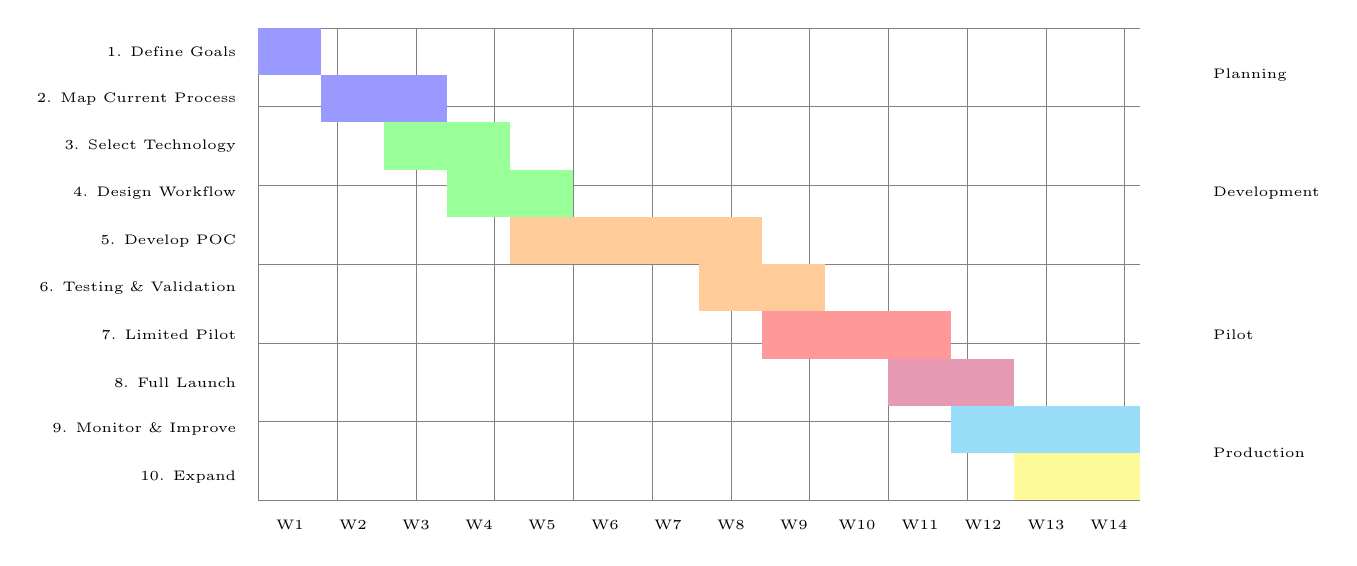
\begin{tikzpicture}[x=0.8cm, y=0.6cm]
% Grid
\draw[step=1cm,gray,very thin] (0,0) grid (14,10);

% Y-axis labels (tasks)
\node[anchor=east, font=\tiny] at (-0.2,9.5) {1. Define Goals};
\node[anchor=east, font=\tiny] at (-0.2,8.5) {2. Map Current Process};
\node[anchor=east, font=\tiny] at (-0.2,7.5) {3. Select Technology};
\node[anchor=east, font=\tiny] at (-0.2,6.5) {4. Design Workflow};
\node[anchor=east, font=\tiny] at (-0.2,5.5) {5. Develop POC};
\node[anchor=east, font=\tiny] at (-0.2,4.5) {6. Testing \& Validation};
\node[anchor=east, font=\tiny] at (-0.2,3.5) {7. Limited Pilot};
\node[anchor=east, font=\tiny] at (-0.2,2.5) {8. Full Launch};
\node[anchor=east, font=\tiny] at (-0.2,1.5) {9. Monitor \& Improve};
\node[anchor=east, font=\tiny] at (-0.2,0.5) {10. Expand};

% X-axis labels (weeks)
\foreach \x in {1,...,14} {
    \node[anchor=north, font=\tiny] at (\x-0.5,-0.2) {W\x};
}

% Gantt bars
\fill[blue!40] (0,9) rectangle (1,10);
\fill[blue!40] (1,8) rectangle (3,9);
\fill[green!40] (2,7) rectangle (4,8);
\fill[green!40] (3,6) rectangle (5,7);
\fill[orange!40] (4,5) rectangle (8,6);
\fill[orange!40] (7,4) rectangle (9,5);
\fill[red!40] (8,3) rectangle (11,4);
\fill[purple!40] (10,2) rectangle (12,3);
\fill[cyan!40] (11,1) rectangle (14,2);
\fill[yellow!40] (12,0) rectangle (14,1);

% Legend
\node[anchor=west, font=\tiny] at (15,9) {Planning};
\node[anchor=west, font=\tiny] at (15,6.5) {Development};
\node[anchor=west, font=\tiny] at (15,3.5) {Pilot};
\node[anchor=west, font=\tiny] at (15,1) {Production};

\end{tikzpicture}
\end{english}
\caption{\en{Gantt Chart} ליישום סוכן אוטונומי -- 14 שבועות}
\label{fig:gantt}
\end{figure}

\section{מתכונים ניהוליים}

\subsection{נוסחה 1: \en{ROI} של אוטומציה}

\[
\text{Automation ROI} = \frac{\text{Saved\_Human\_Hours} \times \text{Hourly\_Wage}}{\text{Dev\_Cost} + \text{Maintenance\_Cost}}
\]

\textbf{\he{דוגמה:}}
\begin{itemize}
    \item \he{חיסכון: 20 שעות/שבוע = 80 שעות/חודש}
    \item \he{שכר שעתי: 150 ש״ח}
    \item \he{עלות פיתוח: 40,000 ש״ח (חד-פעמי)}
    \item \he{עלות תחזוקה: 2,000 ש״ח/חודש}
\end{itemize}

\he{ROI חודשי לאחר החזר השקעה:}
\[
\text{ROI} = \frac{80 \times 150}{40000/12 + 2000} = \frac{12000}{5333} \approx 2.25
\]

\he{כלומר, החל מחודש 4 (לאחר החזר ההשקעה), הסוכן מניב פי 2.25 מהעלות החודשית.}

\subsection{נוסחה 2: שיעור שגיאות}

\[
\text{Error Rate (\%)} = \frac{\text{Errors}}{\text{Total Operations}} \times 100
\]

\textbf{\he{יעדים מומלצים:}}
\begin{itemize}
    \item \he{Tier 1 (פעולות קריטיות): < \en{0.1\%}}
    \item \he{Tier 2 (פעולות חשובות): < \en{1\%}}
    \item \he{Tier 3 (פעולות שגרתיות): < \en{5\%}}
\end{itemize}

\textbf{\he{דוגמה:}}
\he{סוכן שביצע 10,000 פעולות, 47 נכשלו:}
\[
\text{Error Rate} = \frac{47}{10000} \times 100 = 0.47\%
\]

\he{מצוין ל-Tier 2, צריך שיפור ל-Tier 1.}

\subsection{נוסחה 3: \en{Capacity Planning}}

\he{כמה פעולות הסוכן יכול לטפל?}

\[
\text{Max Daily Capacity} = \frac{24 \times 60 \times 60}{\text{Avg\_Execution\_Time}} \times \text{Parallelism}
\]

\textbf{\he{דוגמה:}}
\begin{itemize}
    \item \he{זמן ביצוע ממוצע: \num{30} שניות}
    \item \he{Parallelism: \num{5} (הסוכן יכול להריץ \num{5} משימות במקביל)}
\end{itemize}

\[
\text{Max Capacity} = \frac{86400}{30} \times 5 = 2880 \times 5 = 14,400 \text{ \texthebrew{פעולות/יום}}
\]

\he{בפועל, עם מרווחי ביטחון (\en{80\%} ניצול): 11,520 פעולות/יום.}

\section{תרגילים}

\subsection{תרגיל 1: תכנון סוכן לאוטומציה של משימה יומית}

\textbf{\he{הנחיה:}}
\he{זהה משימה שאתה מבצע באופן קבוע (יומי או שבועי) בעבודתך. תכנן סוכן אוטונומי שיבצע אותה.}

\textbf{\he{מה לכלול:}}
\begin{enumerate}
    \item \he{תיאור המשימה הנוכחית (מה, למה, כמה זמן)}
    \item \he{פירוק לשלבים}
    \item \he{זיהוי מערכות וכלים נדרשים}
    \item \he{אפיון צמתי החלטה}
    \item \he{תכנון טיפול בשגיאות}
    \item \he{הגדרת מטריקות הצלחה}
    \item \he{חישוב ROI משוער}
\end{enumerate}

\subsection{תרגיל 2: השוואה -- \en{n8n} לעומת \en{Make}}

\textbf{\he{הנחיה:}}
\he{חברתך שוקלת לאמץ פלטפורמת אוטומציה. השווה בין n8n ל-Make עבור התרחיש שלכם.}

\textbf{\he{תרחיש:}}
\begin{itemize}
    \item \he{צפי: 50,000 פעולות/חודש}
    \item \he{צורך ב-20 אינטגרציות שונות}
    \item \he{5 workflows מורכבים}
    \item \he{צוות של 3 אנשים (1 טכני, 2 עסקיים)}
    \item \he{רצון לשלוט על הדאטה (שיקולי פרטיות)}
\end{itemize}

\textbf{\he{השווה לפי:}}
\begin{enumerate}
    \item \he{עלות (התחלתית + חודשית)}
    \item \he{קלות יישום}
    \item \he{תמיכה באינטגרציות הנדרשות}
    \item \he{יכולות מתקדמות}
    \item \he{שיקולי אבטחה ופרטיות}
    \item \he{המלצה סופית מנומקת}
\end{enumerate}

\subsection{תרגיל 3: ניתוח כשלון - מה השתבש?}

\textbf{\he{תרחיש:}}
\he{חברת e-commerce השיקה סוכן לניהול מלאי אוטומטי. הסוכן היה אמור להזמין מוצרים כאשר המלאי יורד מתחת לסף. אחרי שבוע:}

\begin{itemize}
    \item \he{\en{30\%} מהמוצרים אזלו ממלאי}
    \item \he{\en{20\%} מהמוצרים הוזמנו בכמויות עודפות}
    \item \he{הסוכן הזמין מוצרים מספקים לא מאושרים}
    \item \he{אף אחד לא קיבל התראה על הבעיות עד שלקוחות התלוננו}
\end{itemize}

\textbf{\he{משימה:}}
\begin{enumerate}
    \item \he{נתח את הכשלים - מה היו הבעיות המהותיות?}
    \item \he{זהה מה חסר בתכנון המקורי}
    \item \he{הצע תיקונים לכל בעיה}
    \item \he{תכנן מנגנוני בקרה שהיו מזהים את הבעיה מוקדם יותר}
\end{enumerate}

\subsection{תרגיל 4: בניית \en{SLA} לסוכן אוטונומי}

\textbf{\he{הנחיה:}}
\he{צור SLA (Service Level Agreement) מפורט עבור סוכן לתמיכת לקוחות.}

\textbf{\he{מה לכלול:}}
\begin{enumerate}
    \item \he{Availability: אחוז זמינות מובטח}
    \item \he{Response Time: זמן תגובה מקסימלי}
    \item \he{Resolution Time: זמן פתרון ממוצע}
    \item \he{Accuracy: אחוז דיוק מינימלי}
    \item \he{Escalation Time: זמן מקסימלי להעברה לאדם}
    \item \he{Error Rate: שיעור שגיאות מקסימלי}
    \item \he{Consequences: מה קורה אם SLA לא מתקיים}
\end{enumerate}

\subsection{תרגיל 5: תכנון הסלמה - מתי סוכן מעביר לאדם?}

\textbf{\he{הנחיה:}}
\he{תכנן מדיניות הסלמה מפורטת עבור סוכן שירות לקוחות.}

\textbf{\he{צור מטריצת החלטות:}}
\begin{table}[h]
\centering
\small
\begin{rtltabular}{|p{3.5cm}|c|c|p{3cm}|}
\hline
\hebheader{תרחיש} & \hebheader{דחיפות} & \hebheader{הסלמה?} & \hebheader{למי?} \\
\hline
\hebcell{בקשת החזר כספי} & \hebcell{בינונית} & \hebcell{כן} & \hebcell{מנהל \textenglish{CS}} \\
\hline
\hebcell{שאלה על מוצר} & \hebcell{נמוכה} & \hebcell{לא} & - \\
\hline
\hebcell{תלונה על עובד} & \hebcell{גבוהה} & \hebcell{כן} & \hebcell{מנהל + \textenglish{HR}} \\
\hline
\hebcell{...} & \hebcell{...} & \hebcell{...} & \hebcell{...} \\
\hline
\end{rtltabular}
\caption{מטריצת החלטות הסלמה}
\label{tab:escalation-matrix}
\end{table}

\textbf{\he{הגדר:}}
\begin{enumerate}
    \item \he{10-15 תרחישים שונים}
    \item \he{עבור כל תרחיש: דחיפות, האם להסלים, למי, תוך כמה זמן}
    \item \he{הגדר טריגרים אוטומטיים (למשל: \en{confidence} < \en{70\%})}
    \item \he{תכנן תהליך \en{handoff} חלק (העברת הקשר לאדם)}
\end{enumerate}

\subsection{תרגיל 6: \en{Python} -- בניית סוכן פשוט עם \en{LangChain}}

\textbf{\he{מטרה:}}
\he{בנה סוכן פשוט שמסוגל לענות על שאלות על חברה מתוך מסמכים.}

\textbf{\he{דרישות:}}
\begin{enumerate}
    \item \he{טען מסמכי PDF או טקסט}
    \item \he{פצל אותם ל-chunks}
    \item \he{צור vector store (FAISS או Chroma)}
    \item \he{בנה agent עם tool לחיפוש במסמכים}
    \item \he{הוסף tool נוסף: מחשבון לחישובים מתמטיים}
    \item \he{תן לסוכן לענות על שאלות תוך שימוש בכלים}
\end{enumerate}

\textbf{\he{קוד בסיס:}}

\begin{english}
\begin{verbatim}
from langchain.agents import initialize_agent, Tool
from langchain.agents import AgentType
from langchain.llms import OpenAI
from langchain.embeddings import OpenAIEmbeddings
from langchain.vectorstores import FAISS
from langchain.document_loaders import PyPDFLoader
from langchain.text_splitter import \
    RecursiveCharacterTextSplitter
from langchain.chains import RetrievalQA

# Load and process documents
def load_documents(pdf_path):
    loader = PyPDFLoader(pdf_path)
    documents = loader.load()

    text_splitter = RecursiveCharacterTextSplitter(
        chunk_size=1000,
        chunk_overlap=200
    )
    texts = text_splitter.split_documents(documents)

    embeddings = OpenAIEmbeddings()
    vectorstore = FAISS.from_documents(texts, embeddings)

    return vectorstore

# Create retrieval QA chain
vectorstore = load_documents("company_docs.pdf")
qa_chain = RetrievalQA.from_chain_type(
    llm=OpenAI(temperature=0),
    chain_type="stuff",
    retriever=vectorstore.as_retriever()
)

# Define tools
tools = [
    Tool(
        name="Company Knowledge Base",
        func=qa_chain.run,
        description="Answers questions about company"
    ),
    Tool(
        name="Calculator",
        func=lambda x: eval(x),  # Use safe eval!
        description="For mathematical calculations"
    )
]

# Initialize agent
agent = initialize_agent(
    tools,
    OpenAI(temperature=0),
    agent=AgentType.ZERO_SHOT_REACT_DESCRIPTION,
    verbose=True
)

# Run
result = agent.run("What is the company's revenue in 2023?")
print(result)
\end{verbatim}
\end{english}

\textbf{\he{משימות נוספות:}}
\begin{enumerate}
    \item \he{הוסף error handling}
    \item \he{הוסף logging}
    \item \he{שמור היסטוריית שיחה}
    \item \he{הגבל מספר צעדים (max\_iterations)}
\end{enumerate}

\subsection{תרגיל 7: \en{Python} -- \en{Workflow} אוטומטי עם \en{Retry} ו-\en{Error Handling}}

\textbf{\he{מטרה:}}
\he{בנה workflow שמטפל בלידים חדשים, כולל retry logic ו-error handling מתקדם.}

\textbf{\he{התהליך:}}
\begin{enumerate}
    \item \he{קבל ליד חדש (JSON)}
    \item \he{אמת את הנתונים}
    \item \he{העשר מ-Clearbit API (עם retry במקרה של כשלון)}
    \item \he{שמור ב-database}
    \item \he{שלח email (עם retry)}
    \item \he{במקרה של כשלון - שלח alert}
\end{enumerate}

\textbf{\he{קוד בסיס:}}

\begin{english}
\begin{verbatim}
import time
import logging
import requests
from typing import Dict, Optional
from dataclasses import dataclass

logging.basicConfig(level=logging.INFO)
logger = logging.getLogger(__name__)

@dataclass
class Lead:
    email: str
    name: str
    company: Optional[str] = None
    title: Optional[str] = None
    enriched: bool = False

class LeadProcessor:
    def __init__(self, max_retries=3, retry_delay=2):
        self.max_retries = max_retries
        self.retry_delay = retry_delay

    def retry_with_backoff(self, func, *args, **kwargs):
        """Generic retry with exponential backoff"""
        for attempt in range(self.max_retries):
            try:
                return func(*args, **kwargs)
            except Exception as e:
                if attempt == self.max_retries - 1:
                    logger.error(f"Max retries reached")
                    raise
                wait = self.retry_delay * (2 ** attempt)
                logger.warning(f"Retry in {wait}s")
                time.sleep(wait)

    def validate_lead(self, lead: Dict) -> Lead:
        """Validate lead data"""
        if not lead.get('email') or '@' not in lead['email']:
            raise ValueError("Invalid email")
        if not lead.get('name'):
            raise ValueError("Name is required")

        return Lead(
            email=lead['email'],
            name=lead['name'],
            company=lead.get('company'),
            title=lead.get('title')
        )

    def enrich_lead(self, lead: Lead) -> Lead:
        """Enrich lead data from Clearbit API"""
        # This is a mock - replace with real API call
        url = "https://api.clearbit.com/v2/people/find"
        response = requests.get(
            f"{url}?email={lead.email}",
            headers={"Authorization": "Bearer API_KEY"},
            timeout=10
        )
        response.raise_for_status()

        data = response.json()
        lead.company = data.get('employment', {}).get('name')
        lead.title = data.get('employment', {}).get('title')
        lead.enriched = True

        return lead

    def save_to_db(self, lead: Lead):
        """Save lead to database"""
        # Mock - replace with real DB logic
        logger.info(f"Saving lead {lead.email} to database")
        # db.leads.insert(lead)
        pass

    def send_email(self, lead: Lead):
        """Send welcome email"""
        # Mock - replace with real email logic
        logger.info(f"Sending email to {lead.email}")
        # email_service.send(to=lead.email...)
        pass

    def send_alert(self, error: str, lead: Dict):
        """Send alert to team"""
        logger.error(f"ALERT: Processing failed - {error}")
        logger.error(f"Lead data: {lead}")
        # In production: send to Slack, etc.

    def process_lead(self, lead_data: Dict):
        """Main workflow"""
        try:
            # Step 1: Validate
            logger.info("Step 1: Validating lead")
            lead = self.validate_lead(lead_data)

            # Step 2: Enrich (with retry)
            logger.info("Step 2: Enriching lead")
            try:
                lead = self.retry_with_backoff(
                    self.enrich_lead, lead
                )
            except Exception as e:
                logger.warning(f"Enrichment failed: {e}")

            # Step 3: Save (with retry)
            logger.info("Step 3: Saving to database")
            self.retry_with_backoff(self.save_to_db, lead)

            # Step 4: Send email (with retry)
            logger.info("Step 4: Sending email")
            self.retry_with_backoff(self.send_email, lead)

            logger.info(f"Processed lead: {lead.email}")

        except ValueError as e:
            logger.error(f"Validation error: {e}")
            self.send_alert(str(e), lead_data)
        except Exception as e:
            logger.error(f"Unexpected error: {e}")
            self.send_alert(str(e), lead_data)
            raise

# Usage
if __name__ == "__main__":
    processor = LeadProcessor(max_retries=3, retry_delay=2)

    # Simulate incoming lead
    new_lead = {
        "email": "john@example.com",
        "name": "John Doe"
    }

    processor.process_lead(new_lead)
\end{verbatim}
\end{english}

\textbf{\he{משימות נוספות:}}
\begin{enumerate}
    \item \he{הוסף circuit breaker pattern (אם API נכשל 5 פעמים ברצף - הפסק לנסות)}
    \item \he{הוסף metrics collection (כמה לידים עובדו, כמה נכשלו, average time)}
    \item \he{הוסף queue לטיפול אסינכרוני בלידים רבים}
    \item \he{בנה dashboard לניטור המערכת}
\end{enumerate}

\section{סיכום: העתיד של עבודת הידע}

\he{המעבר מצ'אטבוטים פשוטים לסוכנים אוטונומיים מלאים איננו רק שדרוג טכנולוגי - זוהי מהפכה בצורה שבה אנו חושבים על עבודה. בפעם הראשונה בהיסטוריה, יש לנו ישויות דיגיטליות שלא רק עונות על שאלות, אלא מתכננות, פועלות, לומדות ומשתפרות.}

\he{עבור מנהלים, זו הזדמנות ואתגר כאחד. ההזדמנות: לשחרר את הצוות שלכם ממשימות שגרתיות וחוזרות, לאפשר להם להתמקד בעבודה יצירתית ואסטרטגית, ולהשיג יעילות תפעולית שלא הייתה אפשרית קודם. האתגר: לעשות זאת באופן מושכל, בטוח, ומבוקר.}

\he{הכלים שסקרנו בפרק זה - מ-LangGraph למפתחים ועד Make ל-zero-code - מנגישים את הטכנולוגיה הזאת לכל ארגון. אינכם צריכים להיות חברת טכנולוגיה ענקית כדי להפעיל סוכנים אוטונומיים. אתם צריכים חשיבה ברורה על התהליכים שלכם, הבנה של היכולות והמגבלות, ונכונות לנסות וללמוד.}

\he{הטעות הגדולה ביותר שארגונים עושים איננה לנסות ולהיכשל - אלא לא לנסות בכלל. העתיד כבר כאן, והוא מתפלג באופן לא שווה. ארגונים שיאמצו את הטכנולוגיה הזאת כעת, יקבלו יתרון תחרותי משמעותי. אלו שיחכו - ימצאו את עצמם מנסים להדביק פער הולך וגדל.}

\he{אבל זכרו: הסוכן האוטונומי הטוב ביותר הוא זה שאתם לא מרגישים. הוא עובד ברקע, מטפל בעבודה השגרתית, ומשחרר את בני האדם לעשות את מה שהם עושים הכי טוב - לחשוב, ליצור, ולקבל החלטות מורכבות שדורשות אמפתיה, יצירתיות, ושיפוט.}

\he{העתיד של העבודה איננו בני אדם נגד מכונות. זהו בני אדם ומכונות, כל אחד עושה את מה שהוא עושה הכי טוב, יחד.}

\vspace{1cm}

\begin{center}
\textbf{\large\he{נקודות המפתח לזכור:}}
\end{center}

\begin{itemize}
    \item \he{סוכן אוטונומי שונה מצ'אטבוט בכך שהוא יוזם, מתכנן, ופועל}
    \item \he{העקרונות המרכזיים: תכנון, ביצוע, למידה, משוב}
    \item \he{קיים מגוון רחב של כלים - מקוד מלא ועד zero-code}
    \item \he{תכנון ה-workflow הוא קריטי להצלחה}
    \item \he{ניטור ובקרה הם לא אופציונליים - הם הכרחיים}
    \item \he{התחילו קטן, למדו, והרחיבו בהדרגה}
    \item \he{מדדו ROI ושפרו באופן מתמיד}
\end{itemize}

\vspace{1cm}

\begin{center}
\he{\textit{"הטכנולוגיה הטובה ביותר היא זו שנעלמת, שמשתלבת בחיי היום-יום עד שהיא בלתי ניתנת להבחנה מהם."}}\\
\he{- מארק וייזר, מדען המחשב שטבע את המושג "Ubiquitous Computing"}
\end{center}
